%%%%%%%%%%%%%%%%%%%%%%%%%%%%%%%%%%%%%%%%%%%%%%%%%%%%%%%%%%%%%%%%%%%%%%%%%%%%%%%%
%Tutorial slides on Python.
%
% Author: FOSSEE
% Copyright (c) 2009, FOSSEE, IIT Bombay
%%%%%%%%%%%%%%%%%%%%%%%%%%%%%%%%%%%%%%%%%%%%%%%%%%%%%%%%%%%%%%%%%%%%%%%%%%%%%%%%

\documentclass[14pt,compress]{beamer}
%\documentclass[draft]{beamer}
%\documentclass[compress,handout]{beamer}
%\usepackage{pgfpages} 
%\pgfpagesuselayout{2 on 1}[a4paper,border shrink=5mm]

% Modified from: generic-ornate-15min-45min.de.tex
\mode<presentation>
{
  \usetheme{Warsaw}
  \useoutertheme{infolines}
  \setbeamercovered{transparent}
}

\usepackage[english]{babel}
\usepackage[latin1]{inputenc}
%\usepackage{times}
\usepackage[T1]{fontenc}

% Taken from Fernando's slides.
\usepackage{ae,aecompl}
\usepackage{mathpazo,courier,euler}
\usepackage[scaled=.95]{helvet}
\usepackage{amsmath}

\definecolor{darkgreen}{rgb}{0,0.5,0}

\usepackage{listings}
\lstset{language=Python,
    basicstyle=\ttfamily\bfseries,
    commentstyle=\color{red}\itshape,
  stringstyle=\color{darkgreen},
  showstringspaces=false,
  keywordstyle=\color{blue}\bfseries}

%%%%%%%%%%%%%%%%%%%%%%%%%%%%%%%%%%%%%%%%%%%%%%%%%%%%%%%%%%%%%%%%%%%%%%
% Macros
\setbeamercolor{emphbar}{bg=blue!20, fg=black}
\newcommand{\emphbar}[1]
{\begin{beamercolorbox}[rounded=true]{emphbar} 
      {#1}
 \end{beamercolorbox}
}
\newcounter{time}
\setcounter{time}{0}
\newcommand{\inctime}[1]{\addtocounter{time}{#1}{\tiny \thetime\ m}}

\newcommand{\typ}[1]{\lstinline{#1}}

\newcommand{\kwrd}[1]{ \texttt{\textbf{\color{blue}{#1}}}  }

%%% This is from Fernando's setup.
% \usepackage{color}
% \definecolor{orange}{cmyk}{0,0.4,0.8,0.2}
% % Use and configure listings package for nicely formatted code
% \usepackage{listings}
% \lstset{
%    language=Python,
%    basicstyle=\small\ttfamily,
%    commentstyle=\ttfamily\color{blue},
%    stringstyle=\ttfamily\color{orange},
%    showstringspaces=false,
%    breaklines=true,
%    postbreak = \space\dots
% }

%%%%%%%%%%%%%%%%%%%%%%%%%%%%%%%%%%%%%%%%%%%%%%%%%%%%%%%%%%%%%%%%%%%%%%
% Title page
\title[Statistics]{Python for Scienc and Engg: Statistics}

\author[FOSSEE] {FOSSEE}

\institute[IIT Bombay] {Department of Aerospace Engineering\\IIT Bombay}

\date[] {08 March, 2010\\Day 1, Session 3}
%%%%%%%%%%%%%%%%%%%%%%%%%%%%%%%%%%%%%%%%%%%%%%%%%%%%%%%%%%%%%%%%%%%%%%

%\pgfdeclareimage[height=0.75cm]{iitmlogo}{iitmlogo}
%\logo{\pgfuseimage{iitmlogo}}


%% Delete this, if you do not want the table of contents to pop up at
%% the beginning of each subsection:
\AtBeginSubsection[]
{
  \begin{frame}<beamer>
    \frametitle{Outline}
    \tableofcontents[currentsection,currentsubsection]
  \end{frame}
}

\AtBeginSection[]
{
  \begin{frame}<beamer>
    \frametitle{Outline}
    \tableofcontents[currentsection,currentsubsection]
  \end{frame}
}

\newcommand{\num}{\texttt{numpy}}


% If you wish to uncover everything in a step-wise fashion, uncomment
% the following command: 
%\beamerdefaultoverlayspecification{<+->}

%\includeonlyframes{current,current1,current2,current3,current4,current5,current6}

%%%%%%%%%%%%%%%%%%%%%%%%%%%%%%%%%%%%%%%%%%%%%%%%%%%%%%%%%%%%%%%%%%%%%%
% DOCUMENT STARTS
\begin{document}

\begin{frame}
  \maketitle
\end{frame}

%% \begin{frame}
%%   \frametitle{Outline}
%%   \tableofcontents
%%   % You might wish to add the option [pausesections]
%% \end{frame}

\section{Computing mean}
\begin{frame}
  \frametitle{Value of acceleration due to gravity?}
  \begin{itemize}
    \item We already have pendulum.txt
    \item We know that $ T = 2\pi \sqrt{\frac{L}{g}} $
    \item So $ g = \frac{4 \pi^2 L}{T^2}  $
    \item Calculate ``g'' - acceleration due to gravity for each pair of L and T
    \item Hence calculate mean ``g''
  \end{itemize}
\end{frame}

\begin{frame}[fragile]
  \frametitle{Acceleration due to gravity - ``g''\ldots}
  \begin{lstlisting}
In []: g_list = []
In []: for line in open('pendulum.txt'):
  ....     point = line.split()
  ....     l = float(point[0])
  ....     t = float(point[1])
  ....     g = 4 * pi * pi * l / (t * t)
  ....     g_list.append(g)
  \end{lstlisting}
\end{frame}

\begin{frame}[fragile]
  \frametitle{Mean ``g'' - Classical method}
  \begin{lstlisting}
In []: total = 0
In []: for g in g_list:
 ....:     total += g
 ....:

In []: g_mean = total / len(g_list)
In []: print 'Mean: ', g_mean
  \end{lstlisting}
\end{frame}

\begin{frame}[fragile]
  \frametitle{Mean ``g'' - Slightly improved method}
  \begin{lstlisting}
In []: g_mean = sum(g_list) / len(g_list)
In []: print 'Mean: ', g_mean
  \end{lstlisting}
\end{frame}

\begin{frame}[fragile]
  \frametitle{Mean ``g'' - One liner}
  \begin{lstlisting}
In []: g_mean = mean(g_list)
In []: print 'Mean: ', g_mean
  \end{lstlisting}
  \inctime{10}
\end{frame}

\section{Processing voluminous data}
\begin{frame}
  \frametitle{More on data processing}
  \begin{block}{}
    We have a huge data file--180,000 records.\\How do we do \emph{efficient} statistical computations, i.e. find mean, median, standard deviation etc; draw pie charts?
  \end{block}
\end{frame}

\begin{frame}
  \frametitle{Structure of the file}
  Understanding the structure of sslc1.txt
  \begin{itemize}
    \item Each line in the file has a student's details(record)
    \item Each record consists of fields separated by ';'
  \end{itemize}
\emphbar{A;015162;JENIL T P;081;060;77;41;74;333;P;;}
\end{frame}

\begin{frame}
  \frametitle{Structure of the file \ldots}
\emphbar{A;015163;JOSEPH RAJ S;083;042;47;AA;72;244;;;}
  Each record consists of:
  \begin{itemize}
    \item Region Code
    \item Roll Number
    \item Name
    \item Marks of 5 subjects: SLang, Flang Maths, Science, Social
    \item Total marks
    \item Pass/Fail (P/F)
    \item Withheld (W)
  \end{itemize}
  \inctime{5}
\end{frame}

\begin{frame}
  \frametitle{Statistical Analysis: Problem statement}
  1. Read the data supplied in the file \emph{sslc1.txt} and carry out the following:
  \begin{itemize}
    \item[a] Draw a pie chart representing proportion of students who scored more than 90\% in each region in Science.
    \item[b] Print mean, median and standard deviation of math scores for all regions combined.
  \end{itemize}
\end{frame}

\begin{frame}
  \frametitle{Problem statement: explanation}
    \emphbar{a. Draw a pie chart representing proportion of students who scored more than 90\% in each region in Science.}
\begin{columns}
    \column{5.25\textwidth}
    \hspace*{.5in}
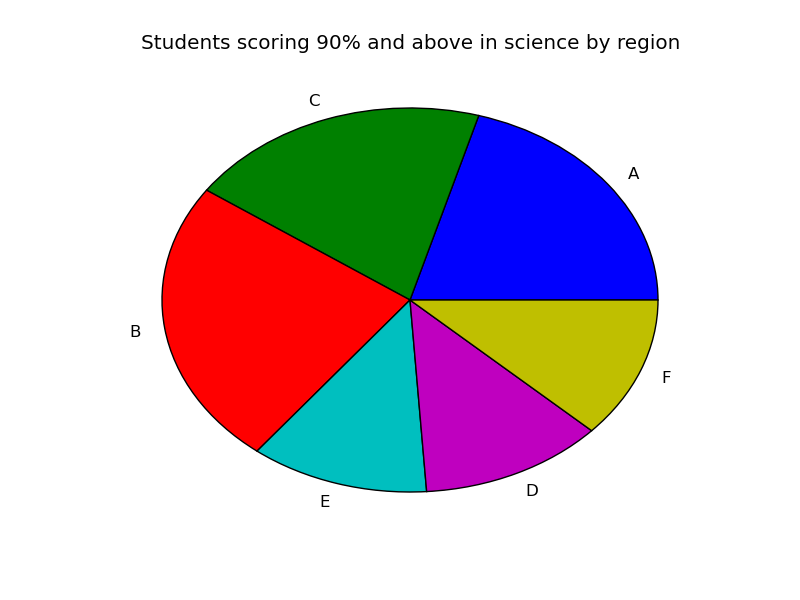
\includegraphics[height=2.6in, interpolate=true]{data/science}
    \column{0.8\textwidth}
\end{columns}
\end{frame}

\begin{frame}
  \frametitle{Machinery Required}
  \begin{itemize}
    \item File reading
    \item Parsing
    \item Dictionaries 
    \item Arrays
    \item Statistical operations
  \end{itemize}
\end{frame}

\subsection{Data processing}
\begin{frame}[fragile]
  \frametitle{File reading and parsing \ldots}
\emphbar{Reading files line by line is the same as we had done with the pendulum example.}

  \begin{lstlisting}
for record in open('sslc1.txt'):
    fields = record.split(';')
  \end{lstlisting}
\end{frame}

\subsection{Dictionaries}
\begin{frame}[fragile]
  \frametitle{Dictionaries: Introduction}
  \begin{itemize}
    \item Lists index using integers\\
Recall \typ{p = [2, 3, 5, 7]} and\\
\typ{p[1]} is equal to \typ{3}
    \item Dictionaries index using strings
  \end{itemize}
\end{frame}

\begin{frame}[fragile]
  \frametitle{Dictionaries \ldots}
  \begin{lstlisting}
In []: d = {'png' : 'image file',
      'txt' : 'text file', 
      'py' : 'python code'
      'java': 'bad code', 
      'cpp': 'complex code'}

In []: d['txt']
Out[]: 'text file'
  \end{lstlisting}
\end{frame}

\begin{frame}[fragile]
  \frametitle{Dictionaries \ldots}
  \begin{lstlisting}
In []: 'py' in d
Out[]: True

In []: 'jpg' in d
Out[]: False
  \end{lstlisting}
\end{frame}

\begin{frame}[fragile]
  \frametitle{Dictionaries \ldots}
  \begin{lstlisting}
In []: d.keys()
Out[]: ['py', 'txt', 'jpg']

In []: d.values()
Out[]: ['python code', 'text file',
       'image file']
  \end{lstlisting}
  \inctime{10}
\end{frame}

\begin{frame}[fragile]
  \frametitle{Getting back to the problem}
  Let our dictionary be:
  \begin{lstlisting}
science = {}
  \end{lstlisting}
\begin{itemize}
    \item Keys will be region codes
    \item Values will be the number students who scored more than 90\% in that region in Science
  \end{itemize}
  \begin{block}{Sample \emph{science} dictionary}
    \{'A': 729, 'C': 764, 'B': 1120,'E': 414, 'D': 603, 'F': 500\}
  \end{block}

\end{frame}

\begin{frame}[fragile]
  \frametitle{Building parsed data \ldots}
  \begin{lstlisting}
science = {}

for record in open('sslc1.txt'):
    fields = record.split(';')

    region_code = fields[0].strip()
  \end{lstlisting}
\end{frame}

\begin{frame}[fragile]
  \frametitle{Building parsed data \ldots}
  \begin{lstlisting}
if region_code not in science:
    science[region_code] = 0

score_str = fields[6].strip()

score = int(score_str) if \
    score_str != 'AA' else 0

if score > 90:
    science[region_code] += 1
  \end{lstlisting}
\end{frame}

\begin{frame}[fragile]
  \frametitle{Building parsed data \ldots}
  \begin{lstlisting}
print science
print science.keys()
print science.values()
  \end{lstlisting}
\end{frame}

\subsection{Visualizing data}
\begin{frame}[fragile]
  \frametitle{Pie Chart}
  \begin{lstlisting}
    pie(science.values())
  \end{lstlisting}
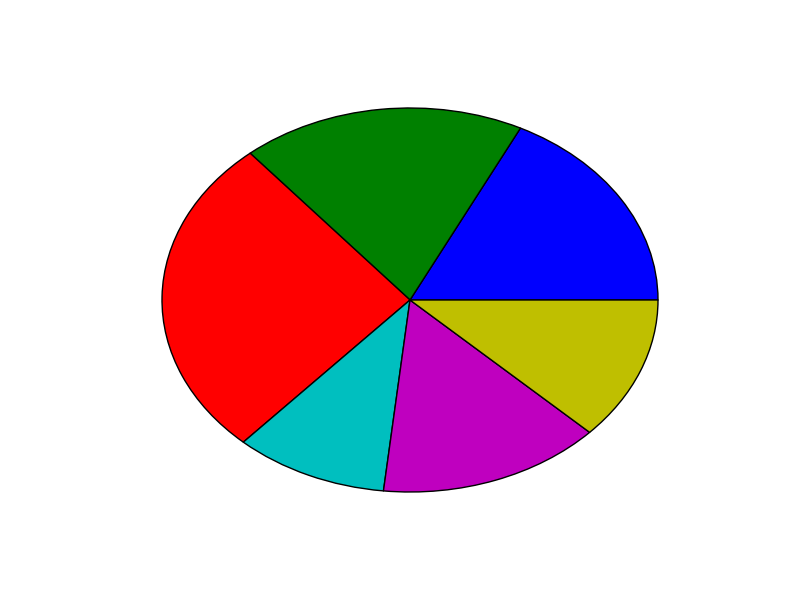
\includegraphics[height=2in, interpolate=true]{data/science_nolabel}
\end{frame}

\begin{frame}[fragile]
  \frametitle{Pie chart}
  \small
  \begin{lstlisting}
pie(science.values(), 
    labels = science.keys())
title('Students scoring 90% and above 
      in science by region')
savefig('science.png')
  \end{lstlisting}
\begin{columns}
    \column{5.25\textwidth}
    \hspace*{1.1in}
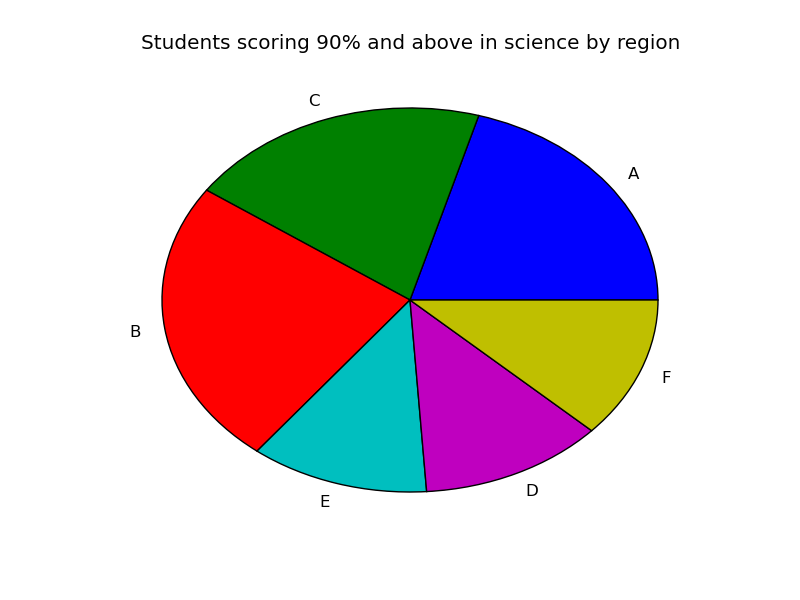
\includegraphics[height=2in, interpolate=true]{data/science}
    \column{0.8\textwidth}
\end{columns}
  \inctime{10}
\end{frame}

\begin{frame}
  \frametitle{Problem statement}
    \emphbar{b. Print mean, median and standard deviation of math scores for all regions combined.}
\end{frame}

\begin{frame}[fragile]
  \frametitle{Building data for statistics}
  \begin{lstlisting}
math_scores = []

for record in open('sslc1.txt'):
    fields = record.split(';')

    score_str = fields[5].strip()
    score = int(score_str) if \
      score_str != 'AA' else 0

    math_scores.append(score)
  \end{lstlisting}
\end{frame}

\subsection{Obtaining statistics}
\begin{frame}[fragile]
  \frametitle{Obtaining statistics}
  \begin{lstlisting}
print 'Mean: ', mean(math_scores)

print 'Median: ', median(math_scores)

print 'Standard Deviation: ',
              std(math_scores)
  \end{lstlisting}
  \inctime{10}
\end{frame}

\begin{frame}[fragile]
  \frametitle{Obtaining statistics: efficiently!}
  \begin{lstlisting}
math_array = array(math_scores)

print 'Mean: ', mean(math_array)

print 'Median: ', median(math_array)

print 'Standard Deviation: ',
              std(math_array)
  \end{lstlisting}
  \inctime{5}
\end{frame}

\begin{frame}[fragile]
  \frametitle{What tools did we use?}
  \begin{itemize}
   \item Dictionaries for storing data
   \item Facilities for drawing pie charts
   \item Efficient array manipulations
   \item Functions for statistical computations - mean, median, standard deviation
  \end{itemize}
\end{frame}

\end{document}

%% Questions for Quiz %%
%% ------------------ %%

\begin{frame}
\frametitle{\incqno }
  A sample line from a Comma Separated Values (CSV) file:\\
  \vspace*{0.2in}
  \emph{Rossum, Guido, 42, 56, 34, 54}\\
  \vspace*{0.2in}
  What code would you use to separate the line into fields?
\end{frame}

\begin{frame}[fragile]
\frametitle{\incqno }
  \begin{lstlisting}
  In []: a = [1, 2, 5, 9]
  \end{lstlisting}
  How do you find the length of this list?
\end{frame}

\begin{frame}[fragile]
\frametitle{\incqno }
  \begin{lstlisting}
  In [1]: d = {
          'a': 1,
          'b': 2
          }
  In [2]: print d['c']
  \end{lstlisting}
  What is the output?
\end{frame}

\begin{frame}[fragile]
\frametitle{\incqno }
\begin{lstlisting}
In []: sc = {'A': 10, 'B': 20, 
             'C': 70}
\end{lstlisting}
Given the above dictionary, what command will you give to plot a
pie-chart?
\end{frame}

\begin{frame}[fragile]
\frametitle{\incqno }
\begin{lstlisting}
In []: marks = [10, 20, 30, 50, 55, 
                75, 83] 
\end{lstlisting}
Given the above marks, how will you calculate the \alert{mean} and
\alert{standard deviation}?
\end{frame}

\begin{frame}[fragile]
\frametitle{\incqno }
\begin{lstlisting}
In []: marks = [10, 20, 30, 50, 55, 
               75, 83] 
\end{lstlisting}
How will you convert the list \texttt{marks} to an \alert{array}?
\end{frame}

%% \begin{frame}[fragile]
%% \frametitle{\incqno }
%%   \begin{lstlisting}
%%   for x in "abcd":
%%       print x

%%   a
%%   b
%%   c
%%   d
%%   \end{lstlisting}
%%   How do you get the following output? 
%%   \begin{lstlisting}
%%     0 a
%%     1 b
%%     2 c
%%     3 d
%%   \end{lstlisting}
%% \end{frame}

